%
% fdm.tex
%
% (c) 2020 Prof Dr Andreas Müller, Hochschule Rapperswil
%
\begin{frame}
\frametitle{Finite Differenzen}
\vspace{-15pt}
\begin{columns}[t]
\begin{column}{0.54\hsize}
\begin{block}{1. Ableitung}
\vspace{-15pt}
\begin{align*}
\frac{\partial u}{\partial x}(x_i,y_i)
&\uncover<2->{\simeq
\frac{u_{i+1,j}-u_{i,j}}{\Delta x}}
\uncover<3->{\simeq
\frac{u_{i,j}-u_{i-1,j}}{\Delta x}}
\\
&
\uncover<4->{\simeq
\frac{u_{i+1,j}-u_{i-1,j}}{2\Delta x}\qquad\text{Leapfrog}}
\end{align*}
\end{block}
\vspace{-15pt}
\uncover<5->{%
\begin{block}{2. Ableitung}
\vspace{-15pt}
\[
\frac{\partial^2 u}{\partial x^2}(x_i,y_k)
\ifthenelse{\boolean{presentation}}{
\only<5>{=
\frac{1}{\Delta x}\biggl(
\frac{u_{i+1,k}-u_{i,k}}{\Delta x}
-
\frac{u_{i,k}-u_{i-1,k}}{\Delta x}\biggr)}
}{}
\only<6->{=
\frac{u_{i+1,k}-2u_{i,k}+u_{i-1,k}}{\Delta x^2}\hspace{20cm}}
%\uncover<7->{=
%\frac{1}{\Delta x^2}(Lu)_{ik}}
\]
\end{block}}
\vspace{-15pt}
\uncover<8->{%
\begin{block}{Laplace-Operator}
Mit $\Delta x=\Delta y = h$:
\[
\Delta u(x_i,y_l)
\simeq
\frac{1}{h^2}(
u_{i-1,l}
+
u_{i+1,l}
+
u_{i,l-1}
+
u_{i,l+1}
-4
u_{i,l})
=
\frac1{h^2}(Lu)_{il}
\]
\end{block}}
\end{column}
\begin{column}{0.42\hsize}
\begin{center}
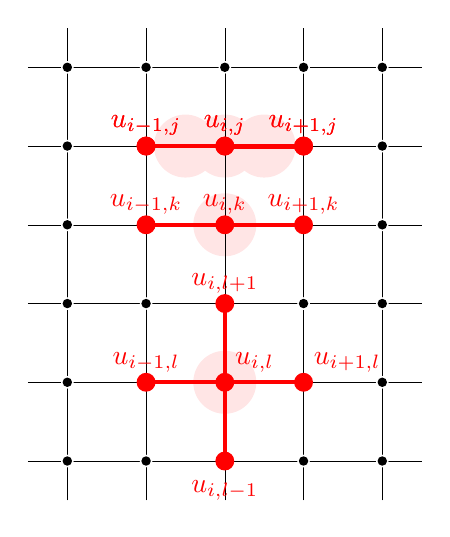
\begin{tikzpicture}[>=latex,thick]

\uncover<2>{
	\fill[color=red!10] (3.5,5) circle[radius=0.4];
}

\uncover<3>{
	\fill[color=red!10] (2.5,5) circle[radius=0.4];
}

\uncover<4>{
	\fill[color=red!10] (3,5) circle[radius=0.4];
}

\uncover<5->{
	\fill[color=red!10] (3,4) circle[radius=0.4];
}

\foreach \x in {1,...,5}{
	\draw[line width=0.2pt] (\x,0.5)--(\x,6.5);
}
\foreach \y in {1,...,6}{
	\draw[line width=0.2pt] (0.5,\y)--(5.5,\y);
}
\foreach \x in {1,...,5}{
	\foreach \y in {1,...,6}{
		\fill[color=white] (\x,\y) circle[radius=0.08];
	}
}

\foreach \x in {1,...,5}{
	\foreach \y in {1,...,6}{
		\fill (\x,\y) circle[radius=0.06];
	}
}

\uncover<2>{
	\draw[color=red,line width=1.8pt] (3,5)--(4,5);
	\fill[color=red] (3,5) circle[radius=0.12];
	\node[color=red] at (3,5) [above] {$u_{i,j}$};
	\fill[color=red] (4,5) circle[radius=0.12];
	\node[color=red] at (4,5) [above] {$u_{i+1,j}$};
}

\uncover<3>{
	\draw[color=red,line width=1.5pt] (2,5)--(3,5);
	\fill[color=red] (2,5) circle[radius=0.12];
	\node[color=red] at (2,5) [above] {$u_{i-1,j}$};
	\fill[color=red] (3,5) circle[radius=0.12];
	\node[color=red] at (3,5) [above] {$u_{i,j}$};
}

\uncover<4->{
	\draw[color=red,line width=1.5pt] (2,5)--(4,5);
	\fill[color=red] (2,5) circle[radius=0.12];
	\node[color=red] at (2,5) [above] {$u_{i-1,j}$};
	\fill[color=red] (4,5) circle[radius=0.12];
	\node[color=red] at (4,5) [above] {$u_{i+1,j}$};
}

\uncover<5->{
	\foreach \x in {2,3,4}{
		\fill[color=red] (\x,4) circle[radius=0.12];
	}
	\draw[color=red,line width=1.5pt] (2,4)--(4,4);
	\node[color=red] at (2,4) [above] {$u_{i-1,k}$};
	\node[color=red] at (3,4) [above] {$u_{i,k}$};
	\node[color=red] at (4,4) [above] {$u_{i+1,k}$};
}

\uncover<8->{
	\fill[color=red!10] (3,2) circle[radius=0.4];
	\fill[color=red] (3,2) circle[radius=0.12];
	\fill[color=red] (2,2) circle[radius=0.12];
	\fill[color=red] (4,2) circle[radius=0.12];
	\fill[color=red] (3,1) circle[radius=0.12];
	\fill[color=red] (3,3) circle[radius=0.12];
	\draw[color=red,line width=1.5pt] (2,2)--(4,2);
	\draw[color=red,line width=1.5pt] (3,1)--(3,3);
	\node[color=red] at (3,2) [above right] {$u_{i,l}\mathstrut$};
	\node[color=red] at (4,2) [above right] {$u_{i+1,l}\mathstrut$};
	\node[color=red] at (2,2) [above] {$u_{i-1,l}\mathstrut$};
	\node[color=red] at (3,1) [below] {$u_{i,l-1}\mathstrut$};
	\node[color=red] at (3,3) [above] {$u_{i,l+1}\mathstrut$};
}

\end{tikzpicture}
\end{center}
\end{column}
\end{columns}

%\begin{columns}[t]
%\begin{column}{0.48\hsize}
%\end{column}
%\begin{column}{0.48\hsize}
%\end{column}
%\end{columns}

\end{frame}
